\Section{StreamIt Programming Language}
\label{sec:streamit}
\vspace{-11pt}

In StreamIt, the basic programmable unit is a {\it filter}.  Each
filter has an independent address space. Thus, all communication with
other filters is via the input and output channels, and occasionally
via control messages (see Section~\ref{sec:messaging}). Each filter
contains a {\it work} function that repeatedly reads data from the
input tape, carries out some computation, and writes data to the
output tape. A filter may also inspect ({\it peek}) data on the input
without removing them. The peek, {\it pop} (read) and {\it push}
(write) rates are declared as part of the work function (see
Figure~\ref{fig:decoder-sj}), thereby enabling the compiler to apply
various optimizations and construct efficient execution schedules.

\begin{figure}[t]
  \center{
 	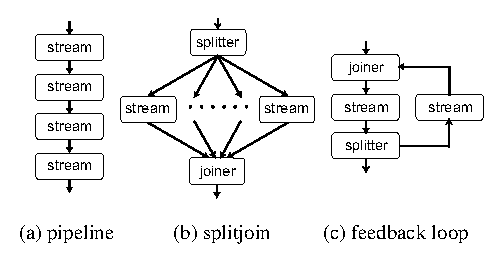
\includegraphics[scale=1, angle=0]{./constructs-eg.eps}
%    \vspace{-11pt}
 	\caption{Hierarchical streams in StreamIt.}
 	\label{fig:containers}
  }
\end{figure}

In StreamIt, the application developer focuses on the hierarchical
assembly of the stream graph and its communication topology, rather
than on the explicit management of the data buffers between filters.
StreamIt provides three hierarchical structures for composing filters
into larger stream graphs (see Figure~\ref{fig:containers}).


\begin{figure}[t]
  \begin{scriptsize}
    \begin{verbatim}
      float->float pipeline IDCT_2D(int N) {
        // N 1D-IDCT in parallel in the X direction
        add splitjoin {
          split roundrobin(N);
          for (int i = 0; i < N; i++)
            add IDCT_1D(N);
          join roundrobin(N);
        }
        // N 1D-IDCTs in parallel in the Y direction
        add splitjoin {
          split roundrobin(1);
          for (int i = 0; i < N; i++)
            add IDCT_1D(N);
          join roundrobin(1);
        }
      }

      float->float filter IDCT_1D(int N) {
        float[N][N] coeff = { ... };
        
        work peek N pop N push N {
          for (int x = 0; x < N; x++) {
            float product = 0;
            for (int u = 0; u < N; u++)
              product += coeff[x][u] * peek(u);
            push(product);
          }
          for (int x = 0; x < N; x++) pop();
        }
      }
    \end{verbatim}
  \end{scriptsize}
  \vspace{-17pt}
  \caption{Example StreamIt code for 2D inverse DCT using two 1D transforms.}
  \vspace{-20pt}
  \label{fig:decoder-sj}
\end{figure}
\begin{figure}[t]
  \begin{scriptsize}
    \begin{verbatim}
      // global variable
      float coeff[64] = { ... };
      
      void IDCT_2D(float* block) {
        int i, j, u;
        float product;
        float tmp[64];
        
        // 1D DCT in X direction
        for (i = 0; i < 8; i++)
          for (j = 0; j < 8; j++) {
            product = 0;

            for (u = 0; u < 8; u++)
              product += coeff[u][j] * block[8*i + u];

            tmp[8*i + j] = product;
          }

        // 1D DCT in Y direction
        for (j = 0; j < 8; j++)
          for (i = 0; i < 8; i++) {
            product = 0;

            for (u = 0; u < 8; u++)
              product += coeff[u][i] * tmp[8*u + j];

            block[8*i + j] = product;
          }
      }
    \end{verbatim}
  \end{scriptsize}
  \vspace{-17pt}
  \caption{Example C code implementation of 2D inverse DCT using two 1D transforms.}
  \vspace{-20pt}
  \label{fig:idct_creference}
\end{figure}

\SubSection{Hierarchical Streams}
\vspace{-11pt}

A {\it pipeline} is a single input to single output parameterized
stream. It composes streams in sequence, with the output of one
connected to the input of the next.  An example of a pipeline appears
in Figure~\ref{fig:decoder-sj}. The {\it splitjoin} construct
distributes data to a set of parallel streams, which are then joined
together in a roundrobin fashion.  StreamIt also provides a {\it
feedback loop} construct for introducing cycles in the graph.

The {\tt add} keyword in StreamIt constructs the specified stream
using the input arguments. The {\tt add} statement may only appear in
non-filter streams.  Filters are the leaves in the hierarchical
construction, and composite nodes define the encapsulating
containers. Thus StreamIt allows for modular design and development of large
applications, thereby  promoting collaboration, increasing code reuse,
and simplifying debugging.

In a splitjoin, the {\it splitter} performs the data scattering, and
the {\it joiner} performs the gathering. A splitter is a specialized
filter with a single input and multiple output channels. On every
execution step, it can distribute its output to any one of its
children in either a {\it duplicate} or a {\it roundrobin} manner.  A
duplicate splitter (indicated by \texttt{split duplicate}) replicates
incoming data to each stream connected to the splitter.  A roundrobin
splitter (indicated by {\tt split roundrobin($w_1,\ldots,w_n$)})
distributes the first $w_1$ items to the first child, the next $w_2$
items to the second child, and so on.  The splitter counterpart is the
joiner.  It gathers data from its predecessors in a roundrobin manner
to produce a single output stream.

The stream constructs provide a convenient and natural way to expose
pipeline parallelism, as well as data parallel streams. The language
also naturally exposes data distribution and communication between
streams. An example is shown in Figure~\ref{fig:decoder-sj}. It
illustrates a parallel implementation of a 2D inverse discrete cosine
transform (DCT) using 1D inverse DCTs. This implementation is both
data parallel (within the rows and columns) and pipeline parallel
(between the rows and columns).  A straightforward C implementation of
a computationally equivalent inverse DCT is shown in
Figure~\ref{fig:idct_creference}. Note that the code structure is
similar to the StreamIt version, although it does not explicitly
expose the parallelism (i.e., parallelization requires loop analysis
and array distribution).  The C code also requires explicit array
index management, such as the  expressions $\texttt{block[8*i+u]}$ and
$\texttt{tmp[8*i+j]}$ which are notably absent in the StreamIt code.
The splitter and joiner in StreamIt free the programmer from tedious
indexing operations, and enable the compiler to understand and
optimize buffer management~\cite{sermulins05lctes}. The StreamIt
implementation is also parameterized such that it is trivial to adjust
the size of the inverse DCT. The equivalent parameterization of the C
code requires adjustments to the loop bounds and array access
expressions.

\SubSection{Teleport Messaging}
\label{sec:messaging}
\vspace{-11pt}

A difficult aspect of stream programming, from both a performance and
programmability standpoint, is reconciling regular streaming dataflow
with irregular control messages.  While the high-bandwidth flow of
data is very predictable, realistic applications also include
unpredictable, low-bandwidth control messages for adjusting
computation parameters (e.g., coefficients used for quantization
during MPEG encoding and decoding).  In StreamIt, such communication
is conveniently accomplished with teleport
messaging~\cite{thies05ppopp}.  The idea behind teleport messaging is
for a message sender to communicate information via asynchronous
method calls to the intended receivers. The method invocations in the
targets are timed relative to the flow of data in the stream. As a
result, teleport messaging avoids muddling data streams with
control-relevant information. In addition, teleport messaging
separates the concerns of the programmer from the system
implementation, thereby allowing the compiler to deliver the message
in the most efficient way for a given architecture: by exposing the
exact data dependences to the compiler, filter executions can be
reordered so long as they respect the message timing. Such reordering
is generally impossible if control information is passed via global
variables.
